\section{Custom Simulator}
The authors developed a custom simulator, shown in Fig.~\ref{fig:simulator_architecture} that supports AXI4, a dual-subnetwork NoC architecture, and three QoS schemes simultaneously. The simulator is built upon the well-known \textit{BookSim2}\TODO{add reference} and \textit{Gem5}\TODO{add reference} frameworks.
The implementation, written in C++, models a system consisting of 168 nodes, two subnetworks, and eight off-chip memory controllers. The design is divided into four identical subareas, each organized as a $7 \times 6$ mesh structure, where every node is connected to a router.
Each node comprises a processor, a private L1 cache, a shared L2 cache, and both a master-side and slave-side network interface (NI). Consequently, every node is capable of functioning simultaneously as a master and a slave. Additionally, each subarea includes two off-chip memory controllers, which are connected to the central routers within the subarea.

\begin{figure}[htbp]
    \centering
    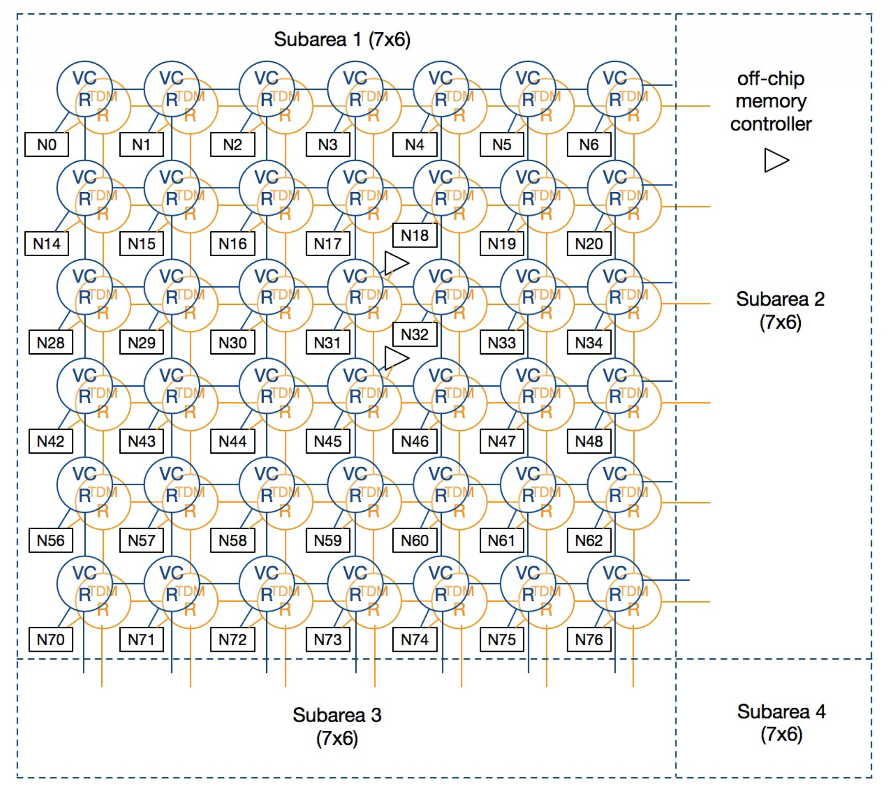
\includegraphics[width=0.95\textwidth]{img/Simulator_Architecture.png.png}
    \caption{Simulator Architecture}~\cite{abderazek_multicore_2013}\label{fig:simulator_architecture}
\end{figure}

The VC network is based on \textit{Gem5}, but for ease of implementation it adopts a cycle-triggered model similar to \textit{BookSim2}, rather than the event-triggered approach used in \textit{Gem5}. The TDM network, by contrast, has a simpler architecture, which facilitates straightforward comparison. 
The network interface (NI) is customized to support the AXI4 protocol. 
Therefore, the results obtained from the proposed simulator can be directly compared with those generated by \textit{Gem5} and \textit{BookSim2}, provided that their NoCs are instantiated with the same configuration.

To regulate the overall injection rate, including LCR, URS, and GRS, the simulator employs a two-level Markov Modulated Process (MMP) model in each traffic generator. The external MMP models the state of a process or thread, whose execution interval varies from nanoseconds to milliseconds. The internal MMP, in turn, models the injection state of request messages during the execution of a process or thread. The parameters $\alpha$ and $\beta$ of the MMP are set according to real-world thread behavior, reflecting both the processing interval and the message injection rate during execution. 

The QoS tag for each request is assigned randomly, based on predefined rates. As a result, a processor is restricted to generating one or two types of QoS schemes, similar to processors in real-world systems. 
The address of each request is also randomly generated from the processor’s communication pairs, which record possible interactions between master and slave nodes. 
Since the influence of the AXI4 ordering requirement is not discussed in this work, the request ID is also selected randomly. This means that ordering constraints may exist for some requests; however, these constraints do not affect the performance of the NoC interconnect, as ordering units are excluded from consideration.

The proposed simulator models a $14 \times 12$ mesh NoC topology, where the average hop count across all requests is four. The TDM period consists of 64 slots (i.e., 64 simulation cycles, one cycle per slot). The VC subnetwork includes two virtual networks, each employing an individual flow control mechanism\TODO{add footnote about alternatives}. 
Each virtual network contains one virtual channel (VC) for LCS packets and one VC for URS packets, with a buffer depth of four flits\TODO{define flit}. The VC router is implemented as a two-stage pipeline, with each stage and each link transfer incurring one cycle of latency. 

The NI can operate at up to 600~MHz in 40-nm technology, but is modeled at 500~MHz in the simulator. To align with the 2~GHz global clock, the NI pipeline latency is scaled from one to four NoC cycles, without impacting subnetwork latency. 
Furthermore, the NI channel width is doubled from 128 to 256 bits, enabling 128~Gb/s throughput, which exceeds the 117~Gb/s maximum throughput requirement of the 2~GHz subnetworks.
